\section{Unsupervised consensus maximization}

Consensus maximization in a set of features related by a geometric constraint that also contains outliers is an important aspect of an SFM system. The problem consists of finding the largest set of inlier features in a set that is consistent with a geometric constraint. In a 3D vision setting the geometric constraint could be for example a rigid transformation $[\textbf{R}\ \textbf{t}]$, a fundamental matrix $F$ or a homography $H$ that relates pairs of corresponding 3D or 2D points.

A popular algorithm to solve this problem is RANSAC\cite{ransac}, but is however not differentiable and therefore not learnable by a neural network. In this paper\cite{consensus} from 2019 the authors present a fully and to end differential method to learn consensus maximization in an unsupervised setting. The explanation  of the method in the paper is however very theoretical and non-accessible to master level students. In this section I will try to explain the method with emphasis on ease of understanding and with the mathematical toolbox of an engineering student.

Consider one of the simplest geometric constraint on a set of corresponding 2D points in subsequent frames of the KITTI dataset, the fundamental matrix $F$. Given a point $u$ in frame 1, and point $v$ in frame 2 they are related in the following way.

 \[
 u^T F v = 0
 \]
 
 To be more explicit the relation can be expressed as follows.
 
\[
\begin{pmatrix}
u_x & u_y & 1 \\
\end{pmatrix}
\begin{pmatrix}
f_{11} & f_{12} & f_{13} \\
f_{21} & f_{22} & f_{23} \\
f_{31} & f_{32} & f_{33} \\
\end{pmatrix}
\begin{pmatrix}
v_x \\
v_y \\
1 \\
\end{pmatrix}
= 0
\]

Multiplication of the two rightmost matrices gives:

\[
\begin{pmatrix}
u_x & u_y & 1 \\
\end{pmatrix}
\begin{pmatrix}
f_{11} v_x + f_{12} v_y + f_{13} \\
f_{21} v_x + f_{22} v_y + f_{23} \\
f_{31} v_x + f_{32} v_y + f_{33} \\
\end{pmatrix}
= 0
\]

Multiplication of the remaining two matrices and grouping the monomials in parentheses for readability gives the following linear equation.

\[
f_{11} (u_x v_x) + f_{12} (u_x v_y) + f_{13} (u_x) +
f_{21} (u_y v_x) + f_{22} (u_y v_y) + f_{23} (u_y) +
f_{31} (v_x) + f_{32} (v_y) + f_{33} (1)
= 0
\]

Now consider a set of M corresponding points that are related by the same fundamental matrix $F$. Place the 9 monomials in the parentheses for all M points in a matrix $ X \in \mathbb{R}^{Mx9} $. A matrix of monomials is called a Vandermonde matrix.

\[
X=
\begin{pmatrix}
u_{x,1} v_{x,1} & u_{x,1} v_{y,1} & u_{x,1} & u_{y,1} v_{x,1} & u_{y,1} v_{y,1} & u_{y,1} & v_{x,1} & v_{y,1} & 1 \\
 & & & \vdots & & & & & \\
u_{x,m} v_{x,m} & u_{x,m} v_{y,m} & u_{x,m} & u_{y,m} v_{x,m} & u_{y,m} v_{y,m} & u_{y,m} & v_{x,m} & v_{y,m} & 1 \\
\end{pmatrix}
\]

The constraint is satisfied by all M points if

\[
X
\begin{pmatrix}
f_{11} \\
f_{12} \\
f_{13} \\
f_{21} \\
f_{22} \\
f_{23} \\
f_{31} \\
f_{32} \\
f_{33} \\
\end{pmatrix}
=
\begin{pmatrix}
0 \\
\vdots \\
0 \\
\end{pmatrix}
^{Mx1}
\]

Now the solution $\textbf{f}$ should look very familiar. The column vector $\textbf{f}$ is in fact the very definition of a nullspace of $X$. This is the key insight in this method of unsupervised consensus maximization. Finding the nullspace of $X$ is done by performing a singular value decomposition (SVD).

\[
U\Sigma V^T=X
\]

The nullspace will be the last column vector of $V \in \mathbb{R}^{9x9}$ and the last singular value $\sigma_9$ in the diagonal of $\Sigma$ will be zero. This is correct only if the set of corresponding points contains only inliers. If the set contains outliers that can not be related by the gemoetric constraint then the last singular value $\sigma_9$ will be greater than zero. If the inliers and outliers where known they could be represented by a vector $\textbf{w} \in [0,1]^m$ where $ 1 $ means inlier and $ 0 $ means outlier. Now $X$ can be weighted by $\textbf{w}$ which would cancel all rows in $X$ which comes from an outlier pair of points.

\[
\diag(\textbf{w}) X \textbf{f} = \textbf{0}
\] 

The problem of finding the largest set of inliers has now been transformed into finding the weights $\textbf{w}$ such that the last singular value $\sigma_9$ of $\diag(\textbf{w})X$ is near zero, and the sum of the weights is large.

To learn the weight $w \in \textbf{w}$ for each pair of points, the PointNet\cite{pointnet} architecture was used. The pair of points are concatenated into rows of a $ X \in \mathbb{R}^{nxm} $ matrix. For 2D points $n = 2+2=4$ and for 3D points $n=3+3=6$. The input $X$ is fed trough the PointNet segmentation network with a single output class, signifying if the point pair is an inlier or not. The key innovation of the PointNet architecture is that it can directly consume point cloud data, as oppose to first transforming the input to a 3D voxel grid or an image. The network is also invariant to the ordering of the points in the input list. Figure \ref{fig:consensus} illustrates the process of feeding the input through pointnet to get the weights, and then applying the weights to the Vandermonde matrix of which we want to minimize the last singular value.

\begin{figure}[H]
	\centering
	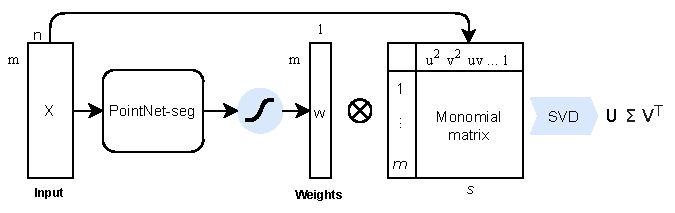
\includegraphics[width=1.0\textwidth]{consensus}
	\caption{}
	\label{fig:consensus}
\end{figure}

Because the fundamental matrix is a constraint expressed by 1 linear equation a basis of only 1  nullspace vector is needed from the singular value decomposition to construct it. But the method can also be used to learn constraints such as a homography or rigid 3D transformation that are constrained by 3 linear equations and therefore require a basis of 3 nullspace vectors.

In the following sections the method used to extract the homography from the basis vectors will be explained. Two points that are related by a homography is expressed as follows.

\[
u \times Hv=0 \rightarrow
\]
\[
[u]_{\times} Hv=0 \rightarrow
\]
\[
\begin{pmatrix}
0 & -1 & u_y \\
1 & 0 & -u_x \\
-u_y & u_x & 0 \\
\end{pmatrix}
\begin{pmatrix}
h_{11} & h_{12} & h_{13} \\
h_{21} & h_{22} & h_{23} \\
h_{31} & h_{32} & h_{33} \\
\end{pmatrix}
\begin{pmatrix}
v_x \\
v_y \\
1 \\
\end{pmatrix}
=
\begin{pmatrix}
0 \\
0 \\
0 \\
\end{pmatrix}
\rightarrow
\]
\[
\begin{cases}
-h_{21} (v_x) \ \ \ \ - h_{22} (v_y) \ \ \ \ - h_{23} (1) \ \ \ + h_{31} (v_x u_y) + h_{32} (v_y u_y) + h_{33} (u_y) = 0 \\
\ \ h_{11} (v_x) \ \ \ \ \ + h_{12} (v_y) \ \ \ \ + h_{13} (1) \ \ -h_{31} (v_x u_x) -h_{32} (v_y u_x) - h_{33} (u_x) = 0 \\
-h_{11} (v_x u_y) -h_{12} (v_y u_y) -h_{13} (u_y) + h_{21} (v_x u_x) + h_{22} (v_y u_x) + h_{23} (u_x) = 0 \\
\end{cases}
\]




